\title{Absorption and Fluorescent Behavior in Ruby Crystal}

\author{William Cutler, Jack Donaghue, Haridas Kumarakuru, Don Heiman}

\newcommand{\abstractText}{\noindent
The unique optical properties of the ruby crystal that make it particularly effective as a lasing medium were measured using an inexpensive setup. Ruby’s absorption of visible light was shown to be strongest at \SI{420}{\nm} and \SI{550}{\nm}, corresponding to its physical appearance as translucent and pink. While the ruby crystal was illuminated with a \SI{532}{\nm} green laser, the R-line fluorescence peaked at \SI{693.8\pm1.1}{\nm}. Finally, the fluorescence lifetime of ruby was measured by pulsing the laser with a signal generator and capturing the decaying light waveform on a digital oscilloscope via a high-speed photodiode. An exponential decay time-constant of \SI{3.6\pm0.1}{\ms} was obtained and will be discussed further in this paper. 
}

%%%%%%%%%%%%%%%%%
% Configuration %
%%%%%%%%%%%%%%%%%

\documentclass[11pt, a4paper, twocolumn]{article}
\usepackage{xurl}
\usepackage[comma,sort&compress]{natbib}
\usepackage{abstract}
\usepackage[separate-uncertainty=true]{siunitx}
\usepackage{graphicx}
\renewcommand{\abstractnamefont}{\normalfont\bfseries}
\renewcommand{\abstracttextfont}{\normalfont\small\itshape}
\usepackage{lipsum}

% Any configuration that should be done before the end of the preamble:
\usepackage{hyperref}
\usepackage{float}
\hypersetup{colorlinks=true, urlcolor=blue, linkcolor=blue, citecolor=blue}
\usepackage[a4paper, total={7in, 10in}]{geometry}
\setlength{\columnsep}{24pt}
\begin{document}
%%%%%%%%%%%%
% Abstract %
%%%%%%%%%%%%

\twocolumn[
  \begin{@twocolumnfalse}
    \maketitle
    \begin{abstract}
      \abstractText
      \newline
      \newline
    \end{abstract}
  \end{@twocolumnfalse}
]

%%%%%%%%%%%
% Article %
%%%%%%%%%%%

\section*{Introduction}
The absorption and fluorescence emission spectra have long been used to identify, characterize, and study materials \cite{BrittanicaSpectroscopy}. In lasing mediums such as ruby, these properties govern its excitation and emission spectra respectively. Studies of ruby absorption typically use a spectrophotometer and measure two broad absorption peaks centered near \SI{410}{\nm} and \SI{550}{\nm} \cite{Esposti,Kusuma,Song}. Devices with high resolution (\SI{0.5}{\nm} slit width) additionally detect a small doublet absorption peak near \SI{694}{\nm}. Song et. al. find absorption peaks at \SI{410}{\nm} and \SI{550}{\nm}, and calculates an absorption coefficient from these values according to Beer-Lambert's law.

The room temperature fluorescence spectrum of ruby has been reported well throughout the early 1900's with a double peak at \SI{692.7}{\nm} and \SI{694.2}{\nm}, corresponding to the characteristic $R_1$ and $R_2$ lines \cite{Kumari, Mani}. With lower resolution instruments, only a single primary peak was detected at \SI{694.2}{\nm} by Esposti et. al. Other fluorescence lines have been detected near these peaks at 671, 688, 695, and \SI{710}{\nm} \cite{Kusuma}.

The effectiveness of ruby as a lasing medium depends on its ability to maintain a population inversion between the ground state and the meta-stable state. The stability of this meta-stable state can be measured by the fluorescence lifetime, which relates to how long the crystal will fluoresce in the absence of pumping, and therefore the time for which there is a size-able meta-stable population. Whereas most materials have nano or picosecond fluorescence lifetimes \cite{Berezin}, ruby’s fluorescence lasts milliseconds, and long enough to hold a population inversion for a working laser.

\begin{figure}
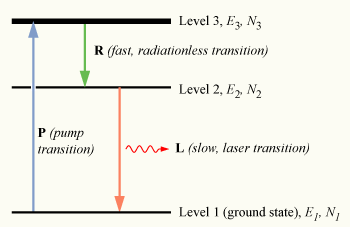
\includegraphics[width=\linewidth]{Population-inversion-3level.png}
\caption{\textit{Sample energy level diagram showing three phases of fluorescence: pumping, non-radiative relaxation, and fluorescent relaxation.}}
\label{fig:populationInversion}
\end{figure}

The fluorescence lifetime of around \SI{3.5}{\ms} is typically reported, but this measurement is dependent on a number of factors. Investigations of the temperature dependence show that lifetime decreases for temperatures above room temperature \cite{Seat, Nelson}. Investigations of the dependence on ruby diameter show an increasing fluorescence lifetime with increased size as emitted photons are reabsorbed more frequently in larger samples \cite{Jones}. The effect of doping concentration changes dramatically with the temperature as found by \cite{Brown}. Brown found that at room temperature, doping concentrations between 0.005\% and 0.1\% yielded lifetimes in the range of 3-\SI{4}{\ms}.

Many investigations use a single-exponential fit to obtain the fluorescence lifetime, but others use a double-exponential fit based on theoretical knowledge and the shape of the residuals for single-exponential fits \cite{McBane, Jones}. There is also some variation on whether a background constant is accounted for, but without it, we found a lifetime further from the typical \SI{3.5}{\ms} and closer to the \SI{4.2}{\ms} reported by Esposti (although it is unclear what actually caused their deviation).

\section*{Results}
\subsection*{Transmission and Absorption}

The transmittance of a material, $T$ is simply the proportion of incident light energy (or intensity) that passes through the material:
\setlength{\abovedisplayskip}{8pt}
\setlength{\belowdisplayskip}{8pt}
$$T=I/I_0$$
$I_0$ represents the incident intensity, and was measured as a function of wavelength by shining a white light into the spectrometer at a particular distance. $I$ is the transmitted intensity, measured using exactly the same setup as $I_0$, but with the ruby crystal in the path between the light and the spectrometer. A black cloth ensured no interference from background light.

\begin{figure}[H]
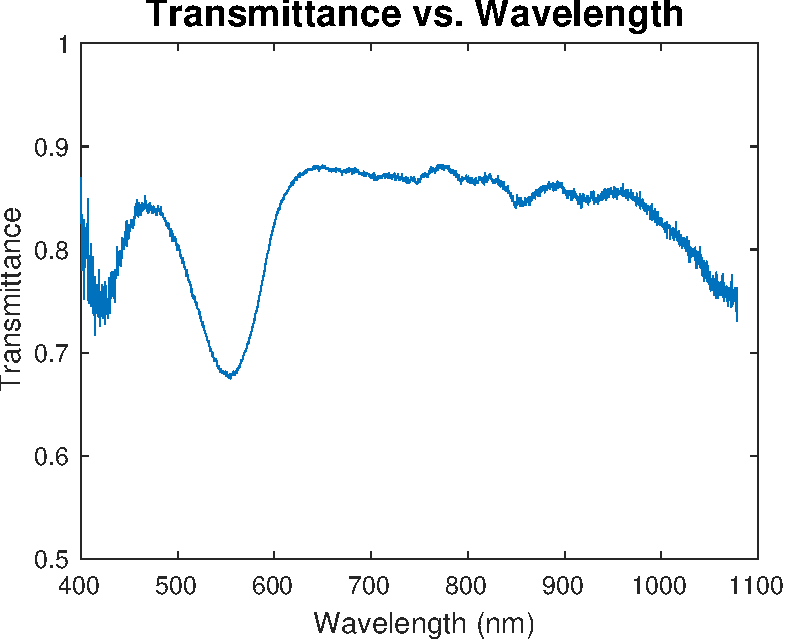
\includegraphics[width=\linewidth]{transmissionSpectrum.pdf}
\caption{\textit{Transmission spectrum of the ruby crystal showing prominent valleys at 420 nm and 550 nm.}}
\label{fig:intensities}
\end{figure}
The reflectivity of the ruby is given by the formula below, and represents the proportion of incident light reflected at one ruby-air interface.
$$R=\frac{(n-1)}{(n+1)}^2$$
The reflectivity can be calculated using a value of $n = 1.780 \pm 0.018$. From these quantities, the absorption coefficient (of the exponential decay of light intensity as it travels along the length of the material) was calculated using:
$$ \alpha = \frac{1}{L}\ln(\frac{I}{I_0}(1-R)^2)$$
Where $L$ is the length of the ruby measured along the path of the light passing through it (thickness). Below are the relevant quantities for calculating the absorption:
\\\\
\begin{tabular}{ll}
\textbf{Index of Refraction} & \textbf{1.780 ± 0.018}    \\
\textbf{Reflectivity}        & \textbf{7.582 ± 0.110\%}  \\
\textbf{Length}              & \textbf{2.00 ± 0.05 mm}  
\end{tabular}
% \begin{figure}[H]
% 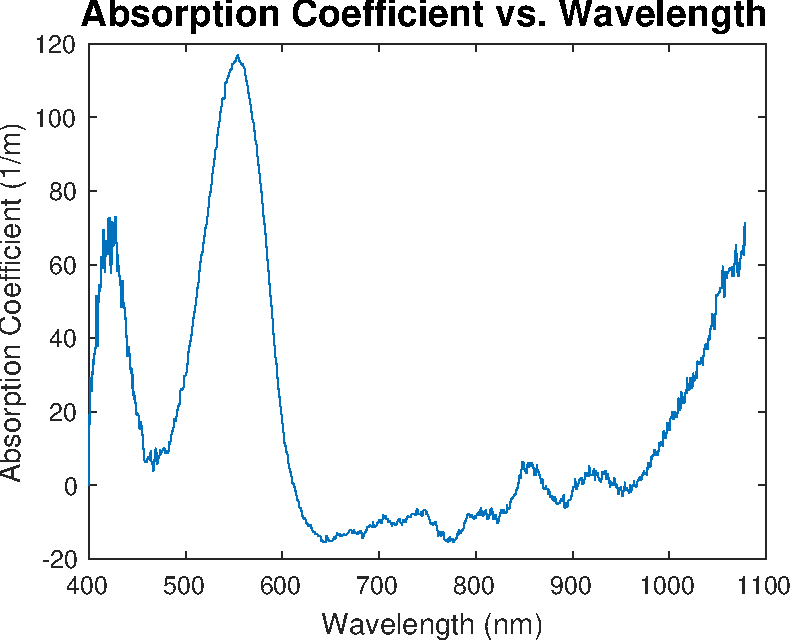
\includegraphics[width=\linewidth]{absorptionSpectrum.pdf}
% \caption{Absorption spectrum of the ruby crystal with two absorption peaks centered at 410 nm and 550 nm}
% \label{fig:intensities}
% \end{figure}
\begin{figure}[]
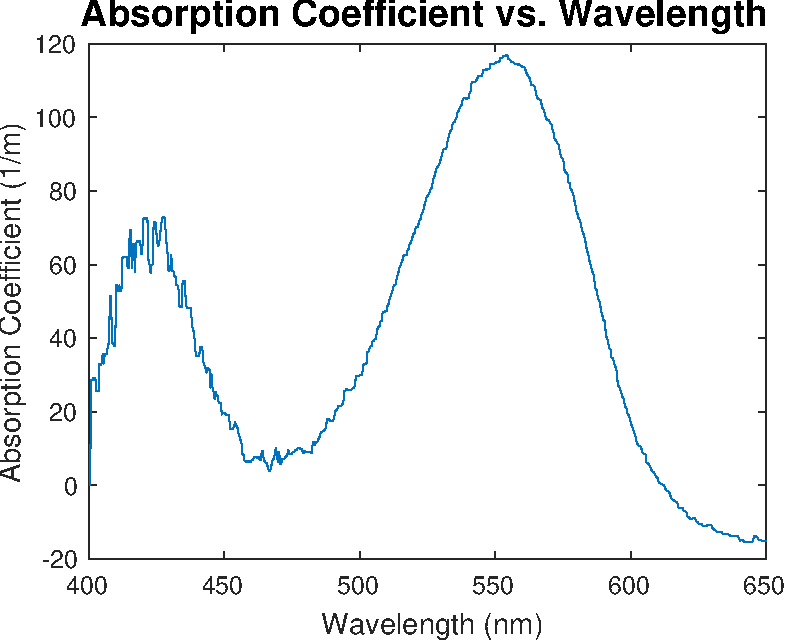
\includegraphics[width=\linewidth]{absorptionSpectrumFocused.pdf}
\caption{\textit{Absorption spectrum focused on the visible light wavelengths showing two broad absorption peaks centered at 410 nm and 550 nm.}}
\label{fig:intensities}
\end{figure}

\begin{figure}[]
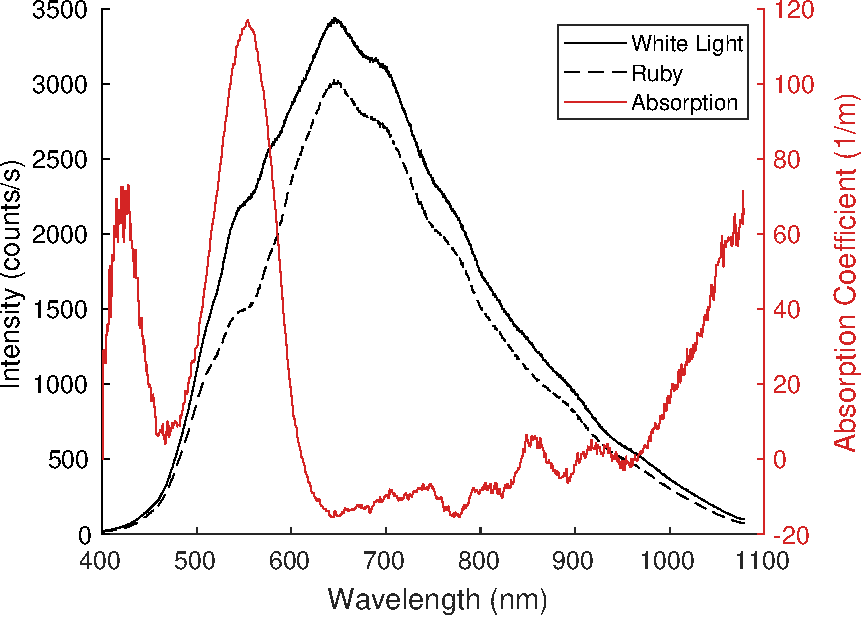
\includegraphics[width=\linewidth]{absorptionAndIntensitySpectra.pdf}
\caption{\textit{Combination of intensity and absorption spectra showing a correspondence between the strongest absorption peak and intensity differential between measurements with and without ruby.}
}
\label{fig:intensities}
\end{figure}

\begin{figure}[]
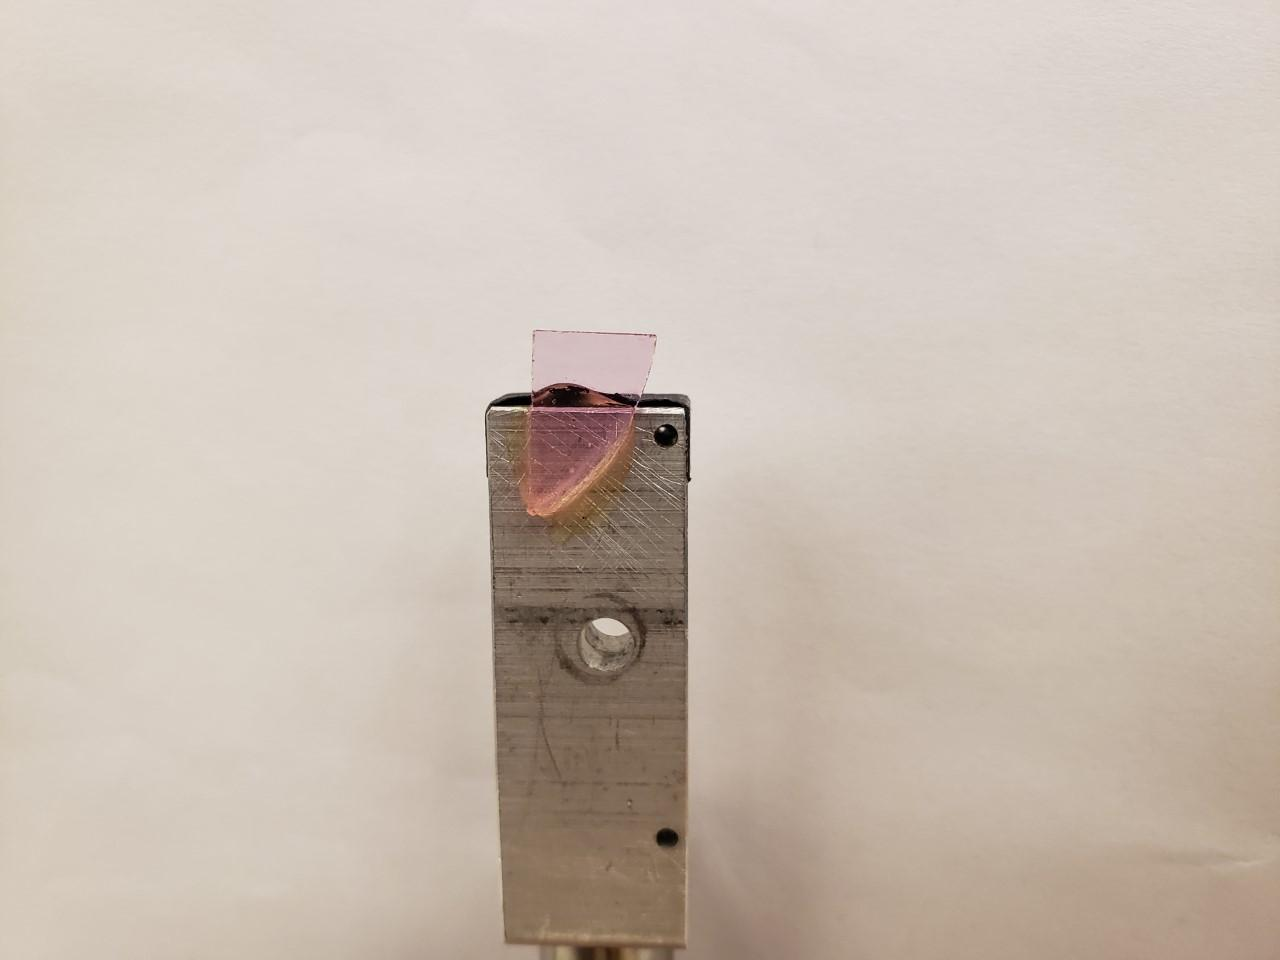
\includegraphics[width=\linewidth]{rubyPhoto.png}
\caption{\textit{Photograph of the transparent pink ruby crystal used throughout this study. Lasers and lights were directed to the top part of the crystal, above the metal stand.}
}
\label{fig:intensities}
\end{figure}

\begin{figure}[]
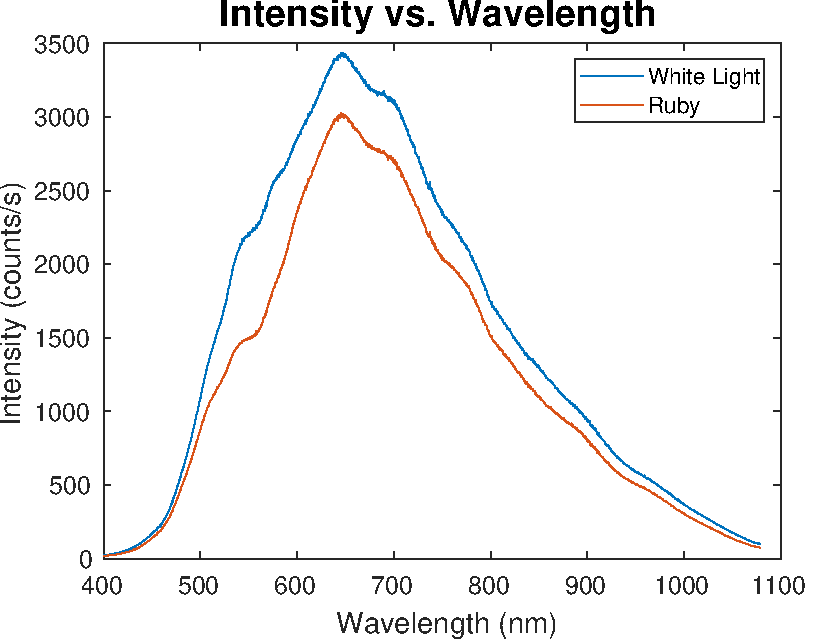
\includegraphics[width=\linewidth]{doubleIntensityMeasurement.pdf}
\caption{\textit{Spectrum of intensities for bare white light and white light passing through ruby.}
}
\label{fig:intensities}
\end{figure}

Because transmittance was recorded as a function of wavelength and other quantities are constant, the absorption coefficient is also a function of wavelength, yielding an absorption spectrum. The absorption showed maxima at 420 ± 5 nm and 553 ± 1 nm wavelengths. These corresponded to absorption coefficients of 66.5 ± 9.9 m$^{-1}$ and 116.7 ± 1.1 m$^{-1}$ respectively. With these values, the intensity of the light would be expected to be reduced by a factor of e after traversing 15.0 ± 2.2 mm and 8.57 ± 0.08 mm respectively. That these lengths are much greater than the actual thickness of the ruby crystal is consistent with the fact that it is mostly transparent. The pink color of the ruby crystal is due to the broad absorption bands of Cr$^{3+}$ in the violet (400 - 450 nm) and yellow-green (500 - 600 nm) regions, with a minimum of absorption in the deep red region ($>$ 650 nm).

\subsection*{Fluorescence Spectrum}
R-line fluorescence was initiated in ruby by directing a constant \SI{532}{\nm} green diode laser beam into the crystal. The resulting fluorescent light was captured by a collection lens and directed through a fiber optic cable to the spectrometer for measurement. A diagram of this setup is shown in Figure \ref{fig:laserBenchDiagram}.
\begin{figure}[]
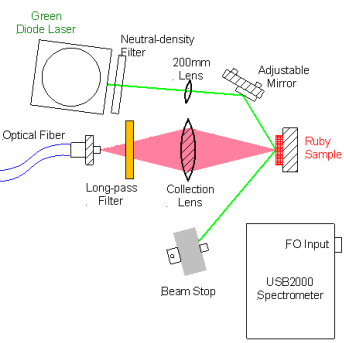
\includegraphics[width=\linewidth]{laserBenchDiagram.png}
\caption{\textit{Diagram of fluorescence spectrum measurement setup showing the laser beam in green and R-line fluorescence in red.}
}
\label{fig:laserBenchDiagram}
\end{figure}
To position the fiber optic mount and focusing lens, a white light was placed at the end of the fiber optic such that its light would pass back through the optic, through the lens, and appear on the ruby sample. Adjustments to the mount and collection lens were made until this light was maximally focused on the ruby, since that would imply the fluoresced light is focused on the fiber optic mount. Additionally, the laser was briefly fired during this adjustment to observe that the focused white light and laser both struck the ruby at the same location. These steps ensured that the fluoresced light that reached the fiber optic was powerful enough to be detected by the spectrometer. 

Peak R-Line fluorescence occurred at 693.5 nm, a deep red color, with a 8 nm FWHM for the entire peak. Although in the visible spectrum, the red fluorescent light itself was not visible due to its low intensity, detectable only by the spectrometer. Because the spectrometer used had a resolution of $>$1 nm, it was unable to discern the double peak found in other experiments, instead showing a single peak spanning the entire double peak range 692.7 to 694.3 nm. Also captured by the spectrometer are smaller peaks on either side of the primary R-line, at 670 nm and 710 nm, corresponding to Neighbor (N) lines and side bands respectively, as detected by Kusuma \cite{Kusuma}.
% \begin{figure}[H]
% 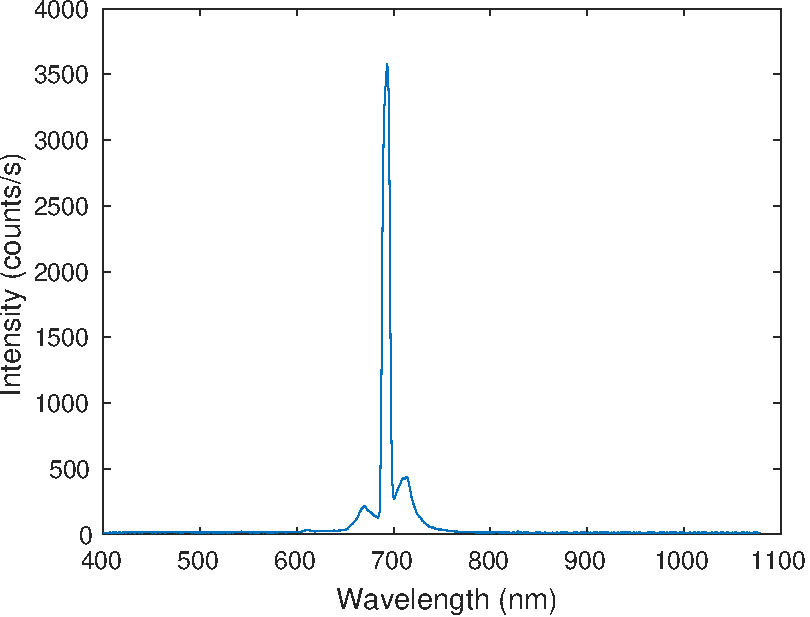
\includegraphics[width=\linewidth]{fluorescenceSpectrum.pdf}
% \caption{Fluorescence spectrum resulting from 532 nm excitation laser showing R-line fluorescence at 693.5 nm}
% \label{fig:intensities}
% \end{figure}
\begin{figure}[]
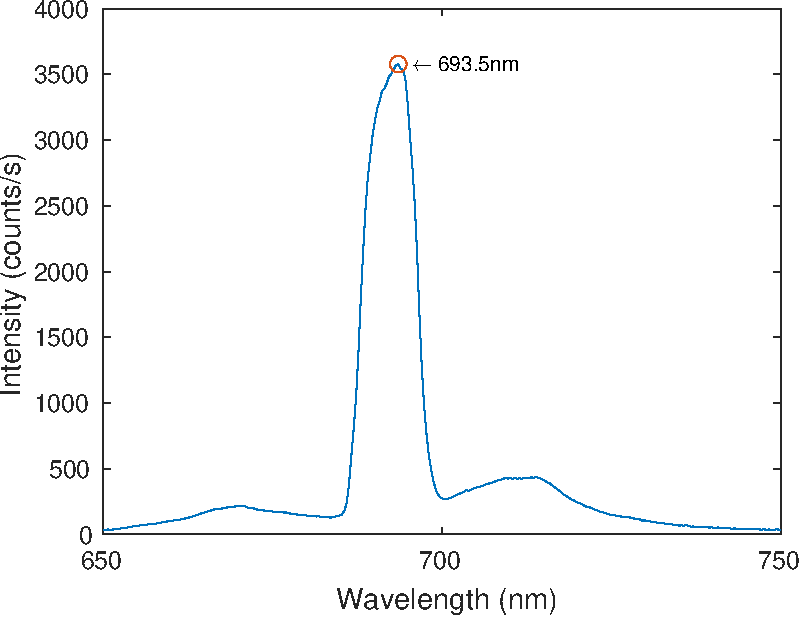
\includegraphics[width=\linewidth]{fluorescenceSpectrumFocused.pdf}
\caption{\textit{Focused fluorescence spectrum showing fluorescence peak.}}
\label{fig:intensities}
\end{figure}

The “efficiency” of the emitted light can be approximated from the ratio of the input wavelength to the output, yielding 532/693.5 = 76.7\%. That is, an R-line fluorescence photon has 76.7\% the energy of the green laser photon absorbed from the relation $E = hc/\lambda$. This is consistent with the non-radiative relaxation step of fluorescence that necessitates that the meta-stable state is of lower energy than the initial excited state.

\subsection*{Fluorescence Lifetime}
Important aspects of the fluorescence process were observed by measuring the strength of fluorescence across time for a ruby crystal subjected to a pulsed laser. The diagram in Figure \ref{fig:decayMeasurementSchematic} shows an abstracted version of the setup and signal path. The laser was pulsed by a 10 Hz square wave function generator and the ruby fluorescence was captured by a photo-diode. An oscilloscope simultaneously recorded the square wave that pulsed the laser (yellow arrow) and the fluorescence signal captured by the photo-diode (blue arrow). A photograph of the laser bench for this process is shown in Figure \ref{fig:laserBenchPhoto}.
\begin{figure}[]
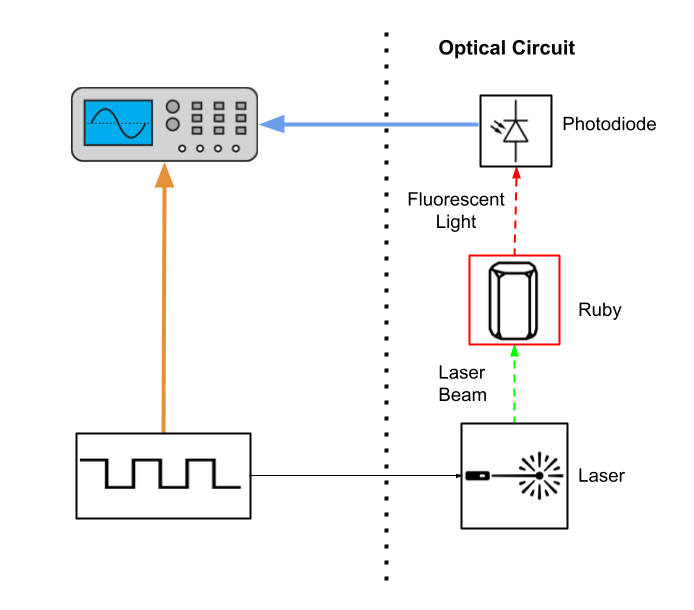
\includegraphics[width=\linewidth]{decayMeasurementSchematic.png}
\caption{\textit{Abstract schematic of fluorescence lifetime measurement showing how the square-wave and the signal path via laser and fluorescence reach the oscilloscope.}}
\label{fig:decayMeasurementSchematic}
\end{figure}

\begin{figure}[]
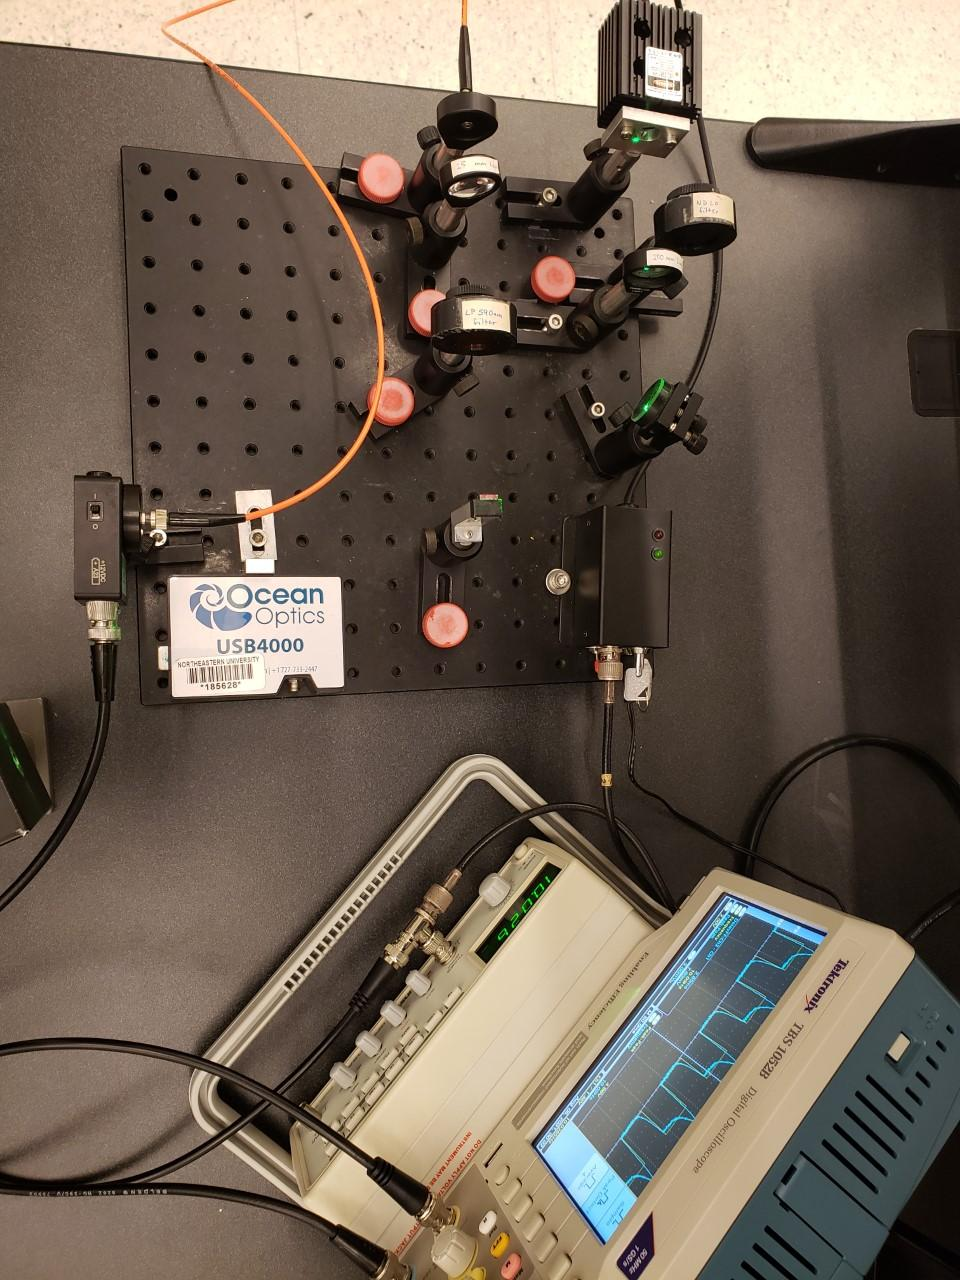
\includegraphics[width=\linewidth, height=\linewidth]{laserBenchPhoto.png}
\caption{\textit{Photograph of laser bench setup for measuring fluorescence lifetime.
}}
\label{fig:laserBenchPhoto}
\end{figure}

The oscilloscope capture of one period of the 10 Hz signal is shown in \ref{fig:fluorescencePeriod}, with the square  wave  in  blue  and  the  fluorescence  in  orange. 
It shows a series of distinct phases outlining the entire process of fluorescence. No fluorescence occurs during the first 0.175 seconds after the laser is fired, indicating a period of laser absorption, chromium excitation, and non-radiative relaxation. The fluorescence rises sharply t = .015 to t = .025, as chromium ions relax back to the ground state. From t = .025 until the laser pulse turns off at t = .05, the rate of fluorescence is saturated, so it does not increase further. Finally, after t = .05, with the laser turned off, fluorescence continues, and the rate of fluorescence decreases exponentially. 

\begin{figure}[]
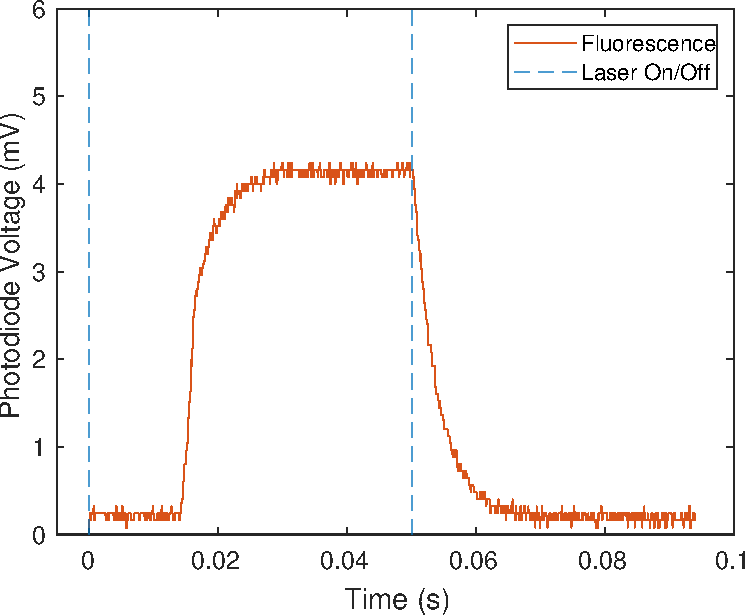
\includegraphics[width=\linewidth]{fluorescencePeriod.pdf}
\caption{\textit{Oscilloscope data for one period of laser pulse at 10 Hz showing the time-correspondence between the laser activation (blue) and measured fluorescence rate (orange).}}
\label{fig:fluorescencePeriod}
\end{figure}

The rate of this exponential decay is governed by the probability that a given meta-stable chromium atom will fluoresce and relax in a given period of time. For the period of time chosen, the smaller this probability of decay, the more stable the meta-stable state is. Using this, the rate of exponential decay can be used to obtain the \textit{fluorescence lifetime} that indicates how stable the R-Line meta-stable state is.

The fluorescence decay was isolated from the oscilloscope data, and a single exponential fit of the form $y = ae^{-x/\tau} + c$ was applied to determine the time constant for the decay, $\tau$, for which a value of \SI{3.6\pm0.1}{\ms} was obtained. The inclusion of a constant in the fit was important because the photo-diode voltage does not decay to 0, but to a background value below 0.5 mV.

\begin{figure}[]
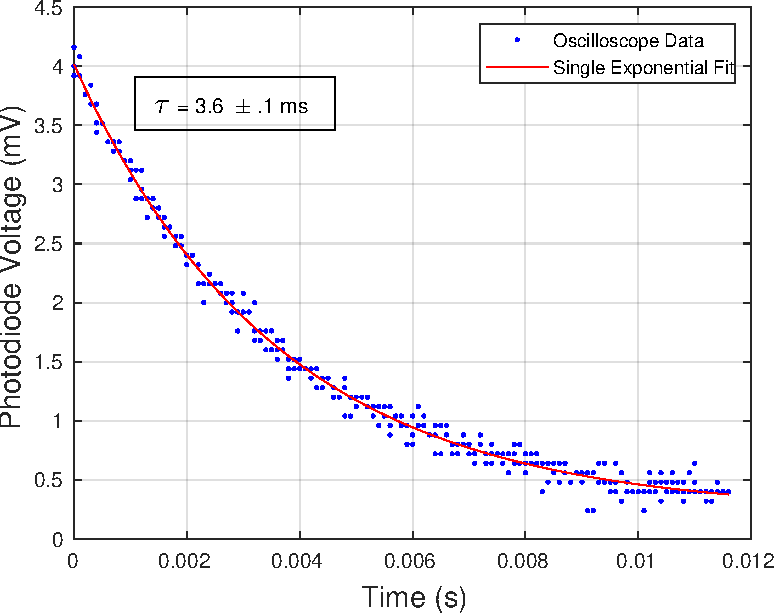
\includegraphics[width=\linewidth]{decayFit.pdf}
\caption{\textit{Exponential curve fit performed in MATLAB to determine the decay constant for fluorescence decay.}
}
\label{fig:populationInversion}
\end{figure}

A single-exponential fit is reported here for its simplicity and interpretability. Furthermore, it provided a high correlation ($R^2 = .993$), and its residual plot, shown in Figure \ref{fig:decayResiduals}, has no discernible pattern, unlike those reported by \cite{Jones} in justification of the double exponential. This is not to deny the theoretical relevance of a double exponential to describing the fluorescence process, but rather to demonstrate that the single exponential fits the data remarkably well beyond mere visual inspection.

\begin{figure}[]
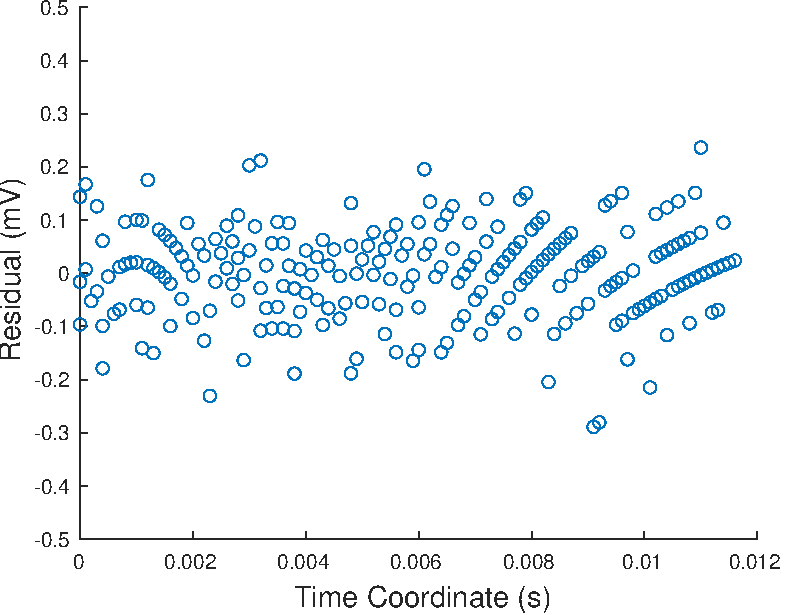
\includegraphics[width=\linewidth]{decayResiduals.pdf}
\caption{\textit{Residual plot for the single exponential fit showing no discernible pattern that might indicate a more complex fit is needed.}}
\label{fig:decayResiduals}
\end{figure}

The time constant represents the amount of time for the fluorescence decay rate to decrease to 1/e of its original value, and is equivalent to the fluorescence lifetime. Whereas many materials exhibit fluorescence lifetimes on the order of ns or ps, ruby’s fluorescence lasts multiple milliseconds, and is a significant factor in its effectiveness as a lasing medium.

\section*{Discussion}
The tests performed concern the optical properties of the ruby crystal sample. The absorption spectrum was found to have peak absorptions at wavelengths of 420 ± 5 nm and 553 ± 1 nm with absorption depths of 15.0 ± 2.2 mm and 8.57 ± 0.08 mm respectively. The transmission and absorption spectra of the ruby were consistent with its visual appearance as a pink translucent crystal. The fluorescence showed a singular clear peak at 693.5 ± 1.1 nm. This range would encompass the double line of the ruby fluorescence spectrum at 692 and 694 nm recorded by (cite source). It also means that the fluorescence has 76.7\% of the energy from the 532nm laser used to excite the ruby. The R-Line fluorescence lifetime was found to be equal to 3.6 ± 0.1 ms.

The results of the experiment would be affected by light from the laboratory if the black cloth used to cover the optic setup were to allow a small amount of light to enter the setup and affect the ruby or spectrometer. Also any dust, oil, or other impurities touching the laser, ruby, spectrometer, or optical component would likewise have changed the measurements and introduced sources of error.

\subsection*{Acknowledgements}
We would like to thank Nathaniel Avish and Hongwei Chen, for their help in the laboratory and as teaching assistants for the Advanced Physics Laboratory section for which this experiment was introduced. We would also like to thank the Northeastern University Department of Physics for supporting our experience at the conference financially.
%%%%%%%%%%%%%%
% References %
%%%%%%%%%%%%%%

\nocite{*}
\bibliographystyle{plain}
\bibliography{reference}

\end{document}

